% !TEX encoding = UTF-8 Unicode
\documentclass[a4paper]{article}

\setcounter{tocdepth}{1}

\usepackage{color}
\usepackage{url}
\usepackage[utf8]{inputenc} % make weird characters work
\usepackage{graphicx}

\usepackage[english]{babel}
%\usepackage[english,serbianc]{babel} %ukljuciti babel sa ovim opcijama, umesto gornjim, ukoliko se koristi cirilica

\usepackage[unicode]{hyperref}
\hypersetup{colorlinks,citecolor=green,filecolor=green,linkcolor=blue,urlcolor=blue}

\usepackage{listings}

%\newtheorem{primer}{Пример}[section] %ćirilični primer
\newtheorem{primer}{Primer}[section]

\definecolor{mygreen}{rgb}{0,0.6,0}
\definecolor{mygray}{rgb}{0.5,0.5,0.5}
\definecolor{mymauve}{rgb}{0.58,0,0.82}

\lstset{ 
  backgroundcolor=\color{white},   % choose the background color; you must add \usepackage{color} or \usepackage{xcolor}; should come as last argument
  basicstyle=\scriptsize\ttfamily,        % the size of the fonts that are used for the code
  breakatwhitespace=false,         % sets if automatic breaks should only happen at whitespace
  breaklines=true,                 % sets automatic line breaking
  captionpos=b,                    % sets the caption-position to bottom
  commentstyle=\color{mygreen},    % comment style
  deletekeywords={...},            % if you want to delete keywords from the given language
  escapeinside={\%*}{*)},          % if you want to add LaTeX within your code
  extendedchars=true,              % lets you use non-ASCII characters; for 8-bits encodings only, does not work with UTF-8
  firstnumber=1000,                % start line enumeration with line 1000
  frame=single,	                   % adds a frame around the code
  keepspaces=true,                 % keeps spaces in text, useful for keeping indentation of code (possibly needs columns=flexible)
  keywordstyle=\color{blue},       % keyword style
  language=Python,                 % the language of the code
  morekeywords={*,...},            % if you want to add more keywords to the set
  numbers=left,                    % where to put the line-numbers; possible values are (none, left, right)
  numbersep=5pt,                   % how far the line-numbers are from the code
  numberstyle=\tiny\color{mygray}, % the style that is used for the line-numbers
  rulecolor=\color{black},         % if not set, the frame-color may be changed on line-breaks within not-black text (e.g. comments (green here))
  showspaces=false,                % show spaces everywhere adding particular underscores; it overrides 'showstringspaces'
  showstringspaces=false,          % underline spaces within strings only
  showtabs=false,                  % show tabs within strings adding particular underscores
  stepnumber=2,                    % the step between two line-numbers. If it's 1, each line will be numbered
  stringstyle=\color{mymauve},     % string literal style
  tabsize=2,	                   % sets default tabsize to 2 spaces
  title=\lstname                   % show the filename of files included with \lstinputlisting; also try caption instead of title
}

\begin{document}

\title{\Large Podrška objektno orijentisanom programiranju u jezicima C++, Objective C, Java, C\#, Ada i Ruby\\ \small{Seminarski rad u okviru kursa\\Metodologija stručnog i naučnog rada\\ Matematički fakultet}}

\author{Katarina Popović, Dušan Pantelić, Dejan Bokić, Nikola Stojević\\ kontakt email prvog, pantelic.dusan@protonmail.com, trećeg, nikolastojevic@gmail.com}

%\date{9.~april 2015.}

\maketitle

\abstract{
U ovom tekstu je ukratko prikazana osnovna forma seminarskog rada. Obratite pažnju da je pored ove .pdf datoteke, u prilogu i odgovarajuća .tex datoteka, kao i .bib datoteka korišćena za generisanje literature. Na prvoj strani seminarskog rada su naslov, apstrakt i sadržaj, i to sve mora da stane na prvu stranu! Kako bi Vaš seminarski zadovoljio standarde i očekivanja, koristite uputstva i materijale sa predavanja na temu pisanja seminarskih radova. Ovo je samo šablon koji se odnosi na fizički izgled seminarskog rada (šablon koji \emph{morate} da koristite!) kao i par tehničkih pomoćnih uputstava. Pročitajte tekst pažljivo jer on sadrži i važne informacije vezane za zahteve obima i karakteristika seminarskog rada.}

\tableofcontents

\newpage

\section{Uvod}
\label{sec:uvod}

\textbf{Programska paradigma} je osnovni stil programiranja, način klasifikovanja programskih jezika na osnovu njihovih karakteristika. Programski jezici (u daljem tekstu jezici) često mogu da se klasifikuju u više od jedne paradigme.

Najčešće programske paradigme su:
proceduralna (fokus stavlja na promenljive), funkcionalna (fokus na matematičkim funkcijama), logička (fokus na logičkim izrazima) i objektno-orijentisana paradigma (fokus je na  \textbf{objektima}). Objekti imaju svoje interno stanje (atribute) i svoje ponašanje (metode).  I metode i atributi mogu a ne moraju biti vidljivi spoljašnjem svetu. Srž objektno-orijentisanog programiranja je u slanju poruka i odgovaranju na njih.  Ovu paradigmu najbolje opisuje  tzv. {\em Tell dont ask} princip- 
\begin{quotation} 
Nemoj da tražiš informaciju koja ti treba da bi uradio posao. Umesto toga, pitaj objekat koji ima tu informaciju da odradi taj posao za tebe. {\em (Allen Hollub- Hollub on Patterns)} 
\end{quotation}
Osnovni principi objektno-orijentisane paradigme:
\begin{enumerate}
\item \textbf{Princip jedinstvene odgovornosti-}  Svaka klasa treba da ima samo jedan zadatak. Čim klasa ima više od jednog zadatka, verovatno bi mogla da se podeli u 2 klase.
\item \textbf{Enkapsulacija-} i {\em Tell dont ask} princip su usko vezani. Vidljivost podataka je osnovni način enkapsulacije. U većini programskih jezika, postoje 3 osnovna nivoa vidljivosti- public, protected i private.
\item \textbf{Nasleđivanje-} podrazumeva da jedna klasa "nasledi" sve metode i atribute svoje nadklase, sem kad su metode i atributi proglašeni privatnim. Uspostavlja odnos "jeste" izmedju klasa- ako klasa A nasleđuje klasu B, kaže se da A "jeste" B. Klasa B se naziva nadklasom klase A. 
Vrste nasleđivanja prikazane su na slici \ref{fig:VrsteNasledjivanja}.
\item \textbf{Polimorfizam-} označava da klase koje implementiraju isti interfejs mogu da rade različite stvari, dok god se drže principa tog interfejsa. 
\item \textbf{Apstrakcija-} je termin koji se veže za {\em interfejse} i {\em apstraktne klase}. \textbf{Interfejsi} se koriste za opisivanje ponašanja klase, definišu javni API (Application programming interface) klase, odnosno metode koje klasa mora da implementira da bi program radio. Oni ne mogu biti instancirani, mogu imati samo potpise metoda, bez tela, ne mogu imati atribute i sve metode moraju biti javne. \textbf{Apstraktne klase} su slične interfejsima, ali za razliku od njih metode apstraktnih klasa mogu da imaju telo, mogu da imaju atribute i mogu imati sva moguća prava pristupa (public, protected, private). 
\end{enumerate}

\begin{figure}[h!]
\begin{center}
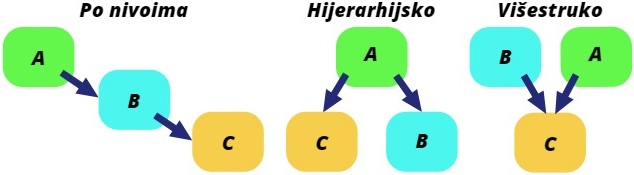
\includegraphics[scale=0.6]{slike/nasledjivanje.jpg}
\end{center}
\caption{Vrste nasledjivanja}
\label{fig:VrsteNasledjivanja}
\end{figure}

\newpage

\section{C++}
\label{sec:c++}
Jezici koji podržavaju sve 4 funkcionalnosti objektno orijentisane paradigme ali ne u potpunosti se obično nazivaju delimično objektno orijentisanim jezicima. Zbog sledećih karakteristika, C++ se smatra delimično objektno orijentisanim jezikom.
\begin{enumerate}
\item \textbf{Main funkcija je izvan klase :} U C++ može da se napiše validan, ispravan kod bez kreiranja ijednog objekta. Main funkcija je obavezna ali se ona nalazi izvan svake klase, što nije karakteristično za druge OOP jezike.
\item \textbf{Koncept globalne promenljive:} U C++ može da se kreira globalna promenljiva koja je dostupna svugde u kodu, dok u drugim OOP jezicima promenljive mogu biti deklarisane samo u okviru klase gde mogu da se koriste modifikatori pristupa (private, protected, public).
\item \textbf{Postojanje friend funkcija:} Friend (prijateljska) funkcija može pristupiti privatnim poljima klase kojoj je deklarisana kao prijateljska. Ovo je jedna veoma korisna karakteristika C++, ali i dalje narušava neke koncepte objektno orijentisane paradigme.
\end{enumerate}

\subsection{Enkapsulacija}
\label{subsec:c++Enkapsulacija}
U C++ ne mora eksplicitno za svaki atribut ili metod klase da bude naglašeno pravo pristupa, nego se prave sekcije, i na početku sekcije se stavi modifikator pristupa (podržani su private, public i protected, ne podržava package modifikator). Ukoliko se modifikator ne navede eksplicitno, kod klasa se podrazumeva private, dok kod struktura se podrazumeva public (što je jedna od osnovnih razlika između struktura i klasa u C++).
\begin{lstlisting}[caption={Primer deklarisanja klase sa enkapsulacijom},frame=single, label=lst:c++Deklaracija]
class Employee {
private:
	int salary;
public: 
	Employee(int e_salary) { salary = e_salary;}
	int getSalary(){ return salary;}
	void setSalary(int newSalary) { salary = newSalary;}
	void display() {
     		std::cout << "Hello I'm the employee!" << std::endl;
	}
};
\end{lstlisting}
\subsection{Nasleđivanje}
\label{subsec:c++Nasledjivanje}
U jeziku C++ i nasleđivanje može biti private, protected ili public. Ukoliko je nasleđivanje public, to znači da sva nasleđena polja ostaju javna, ukoliko je protected, tada ce sva public polja postati protected, a ukoliko je nasleđivanje private, to znači da će sva public i protected polja postati private. Takođe, za razliku od drugih OOP jezika, u C++ je podržano i višestruko nasleđivanje, gde jedna klasa može da nasledi više od jedne klase. Zbog problema koje višestruko nasleđivanje može da uvede, u C++ je uvedena jos jedna ključna reč prilikom nasleđivanja- vritual, koja sprečava tzv. dijamant strukturu. 
\begin{lstlisting}[caption={Primer nasleđivanja klasa u C++},frame=single, label=lst:c++Nasledjivanje]
class Driver: public Employee  {
private:
  	std::string truck = "FAP";
public: 
   	Driver(int salary, std::string truck) 
	: Employee(salary), truck(truck) 
	{};
  	void display() {
		std::cout << "My truck is " << truck << "!" << std::endl; };
};
\end{lstlisting}
\subsection{Polimorfizam}
\label{subsec:c++Polimorfizam}
U C++ su podržana dva osnovna tipa polimorfizma- \textbf{polimorfizam u vreme kompilacije} i \textbf{polimorfizam u vreme izvršavanja}. Prvi obezbeđuje preopterećenje metoda i operatora. Preopterećenje operatora je isto jedna od C++ specifičnih mogućnosti, gde možemo sami da definišemo ponašanje operatora npr "+" dok god ispunjava svoje osnovne karakteristike (da ima 2 argumenta). Drugi tip polimorfizma omogućuje premošćavanje metoda, tj. za metod se kaže da je premošten ukoliko izvedena klasa poseduje metod sa identičnim potpisom. 
\subsection{Apstrakcija}
\label{subsec:c++Apstrakcija}
Za razliku od drugih OOP jezika, C++ ne poseduje ključnu rec ~{\em abstract}. Apstraktne klase se u C++ kreiraju tako što se napravi virtuelna metoda i u potpisu joj se dodeli 0. Takva klasa ne može biti instancirana, ali može biti napravljen pokazivač na nju. Takođe, apstraktna klasa može da ima konstruktor i destruktor. Klasa koje ne premosti virtuelnu metodu takođe postaje apstraktna klasa. Postoji nekoliko pravila koja moraju da važe za apstraktne klase:
\begin{enumerate}
	\item Moraju biti proglašene javnim (inače potklasa ne može da ih premosti).
	\item Virtuelne metode ne mogu biti static i ne mogu biti prijateljske metode neke druge klase.
	\item Virtuelnim metodama se mora pristupati preko pokazivača na baznu klasu da bi se dobio pravi polimorfizam u vreme izvršavanja.
	\item Potpis virtuelne metode mora biti identičan i u baznoj i izvedenoj klasi (povratna vrednost, tipovi argumenata, konstantnost argumenata,...).
	\item Klase mogu imati virtuelni destruktor, ali ne mogu da imaju virtuelni konstruktor.
\end{enumerate}

\section{Objective C}
\label{sec:ObjectiveC}

Proces definisanja klasa se malo razlikuje kod jezika Objective C. Obavlja se u dve sekcije koje se označavaju sa ključnom reči \textbf{@interface} i \textbf{@implementation}, gde se vrši deklaracija i implementacija metoda klase. Obe sekcije se završavaju ključnom reči \textbf{@end}. Svaka klasa je izvedena iz super klase NSObject, čiji konstruktor init je podrazumevani konstruktor, može predefinisati. Moguće je kreirati i svoje konstruktore sa proizvoljnim argumentima,slično ostalim programskim jezicima i mogu se proizvoljno imenovati. Opširnije o ovome u dokumentaciji \cite{ObjectiveCdoc}. U primeru (\ref{ObjectiveC}) vidimo definisanje klase zaposleni (detaljnije \ref{subsec:ObjCEnkapsulacija} ).

\begin{lstlisting}[caption={Primer koda u Objective C jeziku},frame=single, label=ObjectiveC]
@interface Employee : NSObject {
   double salary;	@public int age;
}
@property(nonatomic, readwrite) double salary; 
- (void)display;
@end

@implementation Employee
@synthesize salary; 
- (void)display { NSLog(@"Employee salary is %f", salary); }
@end

@interface Driver : Employee {
   NSString* truck;}
- (id)initWithTruck:(NSString*)model;
@end

@implementation Driver
- (id)initWithTruck:(NSString*)model {
   truck = model;	return self;
   }
- (void)display { NSLog(@"Driver salary is %f", salary); }
@end
int main(int argc, const char * argv[]) {
   NSAutoreleasePool * pool = [[NSAutoreleasePool alloc] init];
   Employee *empl = [[Driver alloc]initWithTruck:@"Mercedes"];
   empl.salary = 5.0;  empl->age = 33;
   [empl display];
   [pool drain];
   return 0;
}}
\end{lstlisting}

\subsection{Enkapsulacija}
\label{subsec:ObjCEnkapsulacija}

Atributi klase su automatski privatni, što pogoduje enkapsulaciji. Njima se omogućuje pristup izvan klase preko ključne reči \textbf{@property}, uz implementaciju pristupnih metoda. Moguće automatsko generisanje metoda pristupa, navođenjem atributa uz ključnu reč \textbf{@synthesize}. Primer(\ref{ObjectiveC}), main funkcija sadrži pozive pristupnim metodama pomoću operatora (.), dok se javnim atributima pristupa preko operatora (->).

\subsection{Nasleđivanje}
\label{subsec:ObjCNasledjivanje}

Ovaj koncept označavamo sa (:) i imenom klase koju nasleđujemo. Primer (\ref{ObjectiveC}), klasa vozač nasleđuje klasu zaposleni .Postoji nasleđivanje u više nivoa i hijerarhijsko. Ako želimo iz izvedene klase da zovemo metode bazne, to radimo referisanjem na baznu klasu pomoću ključne reči \textbf{super}.

\subsection{Polimorfizam}
\label{subsec:ObjCPolimorfizam}

Višestruka upotrebljivost koda u vidu preopterećenosti (eng.~\textbf{\em overloading}) nije omogućeno u Objective C jeziku, tako da se metodi moraju različito imenovati\cite{ObjectiveCbook}. Koncept važnosti metoda(eng.~\textbf{\em overriding})  postoji, i prikazan je u primeru (\ref{ObjectiveC}). Gde klase zaposleni i vozač imaju isti metod display i poziv [empl display] će izvršiti metod klase vozač, zato što promenljiva zaposleni empl referiše na objekat tipa vozač.

\subsection{Apstrakcija}
\label{subsec:ObjCApstrakcija}

Jezik Objective C nema definisan koncept apstraktnih klasa\cite{ObjectiveCbook}, sličan efekat je moguće postići programerskom snalažljivošću i ne instancirati klasu koja bi trebalo biti apstraktna. Za interfejse koje ovde nazivamo protokoli, vezana je ključna reč \textbf{@protocol} jer je \textbf{interface} rezervisana za klase. Sekcija protokola se završava sa \textbf{@end} i može sadžati dve podoblasti \textbf{@required} za metode koji se obavezno moraju implementirati u klasi i \textbf{@optional} za metode čija je implementacija opciona.

\section{Java}
\label{sec:java}

Kako su klase su u centru zbivanja krenućemo od njih. Definišemo ih pomoću ključne reči \textbf{class}. Sledeći primer (\ref{lst:javaDeklaracija}) prikazuje kreiranje klase zaposleni, koja ima svoje atribute i metode(detaljnije \ref{subsec:javaEnkapsulacija}). Objekte klasa instanciramo pomoću metoda konstruktora, koji nema povratni tip i uvek se zove isto kao i klasa. Ako ne definišemo konstruktor, automatski se generiše podrazumevani konstruktor\cite{horstmann2017core}, koji inicijalizuje objekat na podrazumevane vrednosti.

\begin{lstlisting}[caption={Primer deklarisanja klase sa enkapsulacijom i nasleđivanjem},frame=single, label=lst:javaDeklaracija]
public class Employee {
	private int salary;
	#this je referenca na tekuci objekat
	public Employee(int salary) { this.salary = salary;}
 	public int getSalary(){ return salary;}
	public void setSalary(int newSalary) { salary = newSalary;}
	public void display() {
     		System.out.println("Hello i'm employee!");
   }
	public static void main(String[] args) {
    		Employee Marko = new Driver(600,"Mercedes");
    		Marko.display();}    
}
class Driver extends Employee {
  	String truck = "FAP";
	#super vrsi poziv konstruktora bazne klase
   	public Driver(int salary,String truck) {
		super(salary); this.truck = truck;}
  	public void display() {
		System.out.println("My truck is "+truck+"!");
	public void display(String x) {
		System.out.println("My truck is "+truck+x+"!");
}
\end{lstlisting}
\subsection{Enkapsulacija}
\label{subsec:javaEnkapsulacija}

Ograničavanje pristupa internim podacima klase postižemo navođenjem ključne reči ~{\em \textbf{private}} ispred deklaracije promenljive u klasi. Private modifikator pristupa znači da se podacima može pristupiti isključivo iz deklarisane klase. Modifikatori i njihova vidljivost prikazani u tabeli \ref{tab:tabelaModPristupa}. Ako su podaci ipak potrebni van klase, omogućuje se njihovo čitanje i menjanje, preko javnih metode pristupa (eng. ~{\em getters and setters})\cite{horstmann2017core}. U primeru(\ref{lst:javaDeklaracija}), vrednosti privatnog atributa plata možemo pristupiti metodom getSalary() ili menjati sa setSalary(newSalary).

\begin{table}[h!]
\begin{center}
\caption{Vidljivost različitih modifikatora pristupa.}
\begin{tabular}{|l|c|c|c|c|} \hline
Modifikator &Klasa &Paket &Podklasa &Svet\\ \hline
public &Da &Da &Da &Da\\ \hline
protected &Da &Da &Da &Ne\\ \hline
podrazumevani &Da &Da &Ne &Ne\\ \hline
private &Da &Ne &Ne &Ne\\ \hline
\end{tabular}
\label{tab:tabelaModPristupa}
\end{center}
\end{table}

\subsection{Nasleđivanje}
\label{subsec:javaNasledjivanje}

Za nasleđivanje koristimo ključnu reč \textbf{extends}. Obratiti pažnju na primer(\ref{lst:javaDeklaracija}), gde klasa vozač nasleđuje svojstva klase zaposleni. U javi postoji nasleđivanje po nivoima i hijerarhijsko. Višestruko ne postoji direktno\cite{oopJava}, već se implementira preko interfejsa (detaljnije \ref{subsec:javaApstrakcija}).Ako želimo iz izvedene klase da zovemo metode bazne, to radimo referisanjem na baznu klasu pomoću ključne reči \textbf{super}.

\subsection{Polimorfizam}
\label{subsec:javaPolimorfizam}

Višestruka upotrebljivost koda, tj. pripadnost metoda objektu se obavlja u vreme izvršavanja(eng.~{\em run time execution}) i predstavlja koncept važnosti metoda(eng.~{\em\textbf{overriding}})\cite{horstmann2017core}. U primeru koda \ref{lst:javaDeklaracija}, Marko.display(); pozvaće metod klase vozač, iako postoji isti metod bazne klase.

Koncept preopterećenosti metoda(eng.~{\em\textbf{overloading}})\cite{horstmann2017core}, određuje metode u vremenu kompajliranja(eng.{\em compile time}) na osnovu razlika u potpisu metode(različito ime metoda ili tipovi i broj parametara). U primeru koda [\ref{lst:javaDeklaracija}], Marko.display(2); pozvaće metod display(int x) klase vozač.

\subsection{Apstrakcija}
\label{subsec:javaApstrakcija}

Izdvajanje skupa metoda sa kojima spoljašnji korisnik komunicira, prema artiklu \cite{oopJava}, vršimo pomoću apstraktnih klasa ili interfejsa.

Za apstraktne klase navodimo ključnu reč~{\em \textbf{abstract}}(kod \ref{lst:javaAbstract}). Ne mogu se instancirati, ali može biti tip promenljive. Sadrže apstraktne metode(istom ključnom reči obeležavaju) koje treba da predefiniše neka podklasa.

\begin{lstlisting}[caption={Apstraktna klasa},frame=single, label=lst:javaAbstract]
public abstract class Employee {
	public abstract void display(); ...
\end{lstlisting}

Interfejs predstavlja nacrt klase. Sadrži apstraktne, statične, podrazumevane metode(mogu se predefinisati u klasi) i statičke promenljive. Da implementiramo interfejs navodimo ključnu reč~{\em \textbf{implements}}(kod \ref{lst:javaInterfejs}) i zatim ime interfejsa(slično nasleđivanju). Prednost interfejsa\cite{horstmann2017core} je da klasa može implementirati više interfejsa, dok može da nasleđuje samo jednu klasu.

\begin{lstlisting}[caption={Interfejs},frame=single, label=lst:javaInterfejs]
interface Employee {
	public void display(); #podrazumevano apstraktna
	default void work(){System.out.println("Working"); }
\end{lstlisting}


\section{C\#}
\label{sec:csharp}

C\# je jednostavan, moderan, objektno-orijentisan jezik, razvijen od strane Microsoft-a I  odobren od strane ECMA-e(European Computer Manufacturers Association).  Nudi punu podrsku objektno orijentisanom programiranju ukljucujuci nasledjivanje, enkapsulaciju, apstrakciju, I polimorfizam.\\
\\
Ne podrzava druge paradigme ali koristi svoje imperativne strukture. Veome je slicna podrska OOP-u kao kod Java programskog jezika takodje su iste I klase I strukture.\\

\subsection{Enkapsulacija}
\label{subsec:csharpEnkapsulacija}

Enkapsulacija je kada se grupa od povezanih metoda, svojstava I ostalih clanova tretira kao jedan isti objekat.
C\# podrzava sledece specifikatore pristupa:
\begin{itemize}
\item Public:
Dopusta klasi da izlozi varijable i funkcije clanova drugim funkcijama i objektima. Svakom public clanu se moze pristupiti izvan klase.

\item Private:
Dopusta klasi da sakrije promenljive i funkcije clanova od ostalih funkcija i objekata.Samo funkcije iz iste klase mogu pristupiti svojim privatnim clanovima.  Cak i instanca klase ne moze pristupiti svojim privatnim clanovima.\\

\item Protected:
Dopusta podredjenoj klasi da pristupi  varijablama i funkcijama clanova svoje osnovne klase. Na taj nacin pomaze u implementiranju nasledjivanja.\\

\item Internal:
Dopusta klasi da izlozi varijable i funkcije clanova drugim funkcijama i objektima u trenutnom skupu. Tacnije svakom clanu sa ovim specifikatorom pristupa se moze pristupiti iz bilo koje klase ili metode definisane unutar aplikaciju u kojoj je definisan clan.\\

\item Protected internal:
Dopusta klasi da sakrije promenljive i funkcije clanova od ostalih funkcija i objekata klase, osim podredjene klase unutar iste aplikacije.To se takodje koristi kod implementacije nasledjivanja.\\
\end{itemize}

\subsection{Nasledjivanje}
\label{subsec:csharpNasledjivanje}

Nasledjivanje je, kao sto samo ime kaze, mogucnost da “nasledjuje” metode I svojstva od postojecih klasa.\\
Kod c\# nasledjivanja, klasa ciji su clanovi nasledjeni se zove bazicna (roditeljska) klasa, a klasa koja nasledjuje clanove bazicne klase se zove izvedena (podredjena) klasa.\\
C\# Koristi sintaksu c++ za definisanje klasa.\\
Nasledjena metoda od roditeljske klase moze biti zamenjena u izvedenoj klasi tako sto se definise kao new(novo).\\
Verzija roditeljske klase se I dalje moze zvati eksplicitnom sa prefiksom base(baza): base.Draw().\\

\subsection{Polimorfizam}
\label{subsec:csharpPolimorfizam}

U c\#-u, polimorfizam omogucava klasama da da implementiraju razlicite metode koje se nazivaju istim imenom i omogucava pozivanje metoda izvedene klase kroz referencu bazicne klase tokom izvodjena, na osnovu nasih zahteva.\\
U c\#-u imamo dve razlicite vrste polimorfizma a to su: Polimorfizam vremena kompiliranja i polimorfizam vremena izvodjenja.\\

\subsection{Apstrakcija}
\label{subsec:csharpApstrakcija}

Apstrakcija je proces kod koga programer krije sve osim relevantnih podataka o datom objektu u cilju pojednostavljanja I povecanja efikasnosti.\\
U c\#-u mozemo napraviti klasu sa potrebnim metodama i svojstvima i mozemo izloziti samo potrebne metode i svojstva koristeci modifikatore pristupa na osnovu nasih zahteva. \\

\begin{lstlisting}[caption={Primer deklarisanja apstraktivne klase u C\#-u},frame=single, label=lst:csharpDeklaracija]
abstract class MobilePhone {  
    public void Calling();  
    public void SendSMS();  
}  
public class Nokia1400: MobilePhone {}  
public class Nokia2700: MobilePhone {  
    public void FMRadio();  
    public void MP3();  
    public void Camera();  
}  
public class BlackBerry: MobilePhone {  
    public void FMRadio();  
    public void MP3();  
    public void Camera();  
    public void Recording();  
    public void ReadAndSendEmails();  
} 
\end{lstlisting}

\section{Ada}
\label{sec:ada}

Ada sledi model klase zasnovan na odvojenim karakteristikama (tipovima(eng. ~{\em types}) deklarisanim u jedinicama paketa(eng. ~{\em package})), a ne na jednom konstruktoru klase\cite{oopAda}. Klasa u Adi ima koncept klase tipa koja se sastoji od skupa tipova kreiranih unutar deklaracije osnovnog tipa(eng. ~{\em root type}) unutar paketa. Svakom tipu je pridružena oznaka(eng. ~{\em tag}) koja ga razlikuje od ostalih tipova dodavanjem ključne reči \textbf{tagged} u deklaraciju osnovnog tipa. Unutar paketa možemo imati procedure(nemaju povratnu vrednost) i funkcije(imaju povratnu vrednost). U nastavku možemo videti primer(\ref{lst:adaDeklaracija}) OOP u Adi.

\begin{lstlisting}[caption={Primer objektno orijentisanog programiranja u jeziku Ada.},frame=single, label=lst:adaDeklaracija]
package Employees is 
	type Employee is tagged 
	record
		Name: String;
	end record;
	procedure Set_Name(Obj: in out Employee; Name: Name_Type);
end Employees;
package Drivers
type Driver is new Employees.Employee with record
	null;
end record;
\end{lstlisting}

\subsection{Enkapsulacija}
\label{subsec:adaEnkapsulacija}
U Adi, enkapsulacija je malo drugačija od većine OOP jezika jer je privatnost generalno određena na nivou paketa\cite{adaIntroduction}. Pomoću ključne reči \textbf{private} u deklaraciji baznog tipa obezbeđujemo da podacima unutar tipa pristupamo jedino pomoću funkcija i procedura. Još veći stepen privatnosti dobijamo dodavanjem ključne reči \textbf{limited} ispred ključne reči \textbf{private}. Procedure i funkcije unutar paketa deklarišemo kao privatne ukoliko ispred niza deklaracija procedura i funkcija dodamo ključnu reč \textbf{private}.

\subsection{Nasleđivanje}
\label{subsec:adaNasledjivanje}
Nasleđivanje po nivoima i hijerarhijsko nasleđivanje je direktno podržano u Adi, dok je višestruko nasleđivanje moguće implementirati pomoću interfejsa(eng. ~{\em interface}) uz dodatni rad programera. U primeru(\ref{lst:adaDeklaracija}) deklaracija klase \textit{Driver} je tipičan primer kreiranja izvedenog tipa. Izvedeni tip nasleđuje sve podatke unutar tipa, kao i sve procedure i funkcije rodjiteljskog tipa.

\subsection{Polimorfizam}
\label{subsec:adaPolimorfizam}

\subsection{Apstrakcija}
\label{subsec:adaApstrakcija}

\section{Ruby}
\label{sec:ruby}
 Podršku u programskom jeziku Ruby ilustrovaćemo primerom(\ref{lst:rubyDeklaracija}) koji pokriva sve bitnije aspekte objektno orijentisanog programiranja. Standardni metod klase je \textbf{initialize}, on se poziva automatski prilikom kreiranja objekta i ponaša se skoro identično kao konstruktori u drugim programskim jezicima.

\begin{lstlisting}[caption={Primer objektno orijentisanog programiranja u jeziku Ruby.},frame=single, label=lst:rubyDeklaracija]
class Employee
attr_accessor :name
def initialize(name)
	@name = name
	print()
end
def print
	puts "Employee: #{@name}."
end
end
class Driver < Employee
	def initialize(name)
		@name = name
		print()
	end
	private
	def print
		puts "Driver: #{@name}."
	end
end

emp = Employee.new("John")
drv = Driver.new("John")
\end{lstlisting}

\subsection{Enkapsulacija}
\label{subsec:rubyEnkapsulacija}
Kako u samom jeziku ne postoji mogućnost direktnog pristupa podacima unutar klase(podaci su privatni), njima možemo pristupiti jedino pomoću metoda klase. Svi metodi klase su javni, osim ako nije eksplicitno naznačeno drugačije ključnim rečima \textbf{public} \textbf{protected}, \textbf{private} neposredno pre definicije jednog ili više metoda. Ruby nam pruža mogucnost ugrađenih metoda za pristup(eng. ~{\em accessor methods}). U primeru(\ref{lst:rubyDeklaracija})  \textbf{attr\_accessor} omogućava čitanje i menjanje vrednosti promenljivih klase. Pomocu \textbf{attr\_reader} i \textbf{attr\_writer} možemo pojedinačno dopustiti samo čitanje odnosno samo menjanje vrednosti promenljivih.

\subsection{Nasleđivanje}
\label{subsec:rubyNasledjivanje}
Kada nakon imena klase u njenoj definicije dodamo znak < za kojim sledi ime već postojeće klase, dobijamo efekat nasleđivanja koji možemo videti u prethodnom primeru(\ref{lst:rubyDeklaracija}) gde klasa \textit{Driver} nasleđuje klasu \textit{Employee}(primetiti da u klasi \textit{Driver} nismo implementirali \textbf{attr\_accessor} jer se nasledjuje). Nasleđivanje po nivoima i hijerarhijsko nasleđivanje je moguće dok višestruko nasleđivanje nije(više o tipovima nasleđivanja u \ref{subsec:javaNasledjivanje}).

\subsection{Polimorfizam}
\label{subsec:rubyPolimorfizam}
Osnovni vid polimorfizma možemo postići nasleđivanjem tako sto ce razliciti objekti odgovoriti različito na iste metode. U primeru(\ref{lst:rubyDeklaracija}) u klasi \textit{Driver} smo definisali metod \textit{print} koji je istog naziva kao i nasleđeni metod čime postižemo da instanca klase odgovori različito na metod od instance roditeljske klase. 

Drugačiji vid polimorfizma postižemo takozvanim "pačijim kucanjem"(eng. ~{\em duck typing}) u kojem nisu bitni tipovi objekata već skup istoimenih metoda koje poseduju. Za primer uzmimo klasu \textit{Duck} koja poseduje metod  \textit{quack} i funkciju koja za argument uzima objekat tipa \textit{Duck} i poziva metod \textit{quack}. U tom slučaju funkciji možemo proslediti bilo koji objekat koji poseduje metod naziva \textit{quack}(sa istim ili različitim ponašanjem metoda) i gledati na njega kao da je tipa \textit{Duck} bez obzira što on to nije.

\subsection{Apstrakcija}
\label{subsec:rubyApstrakcija}
Ruby nema direktnu podršku za apstrakciju klasa ali se sličan efekat može dobiti korišćenjem biblioteke "abstract". Takođe je moguće implementirati apstakciju pomoću nasleđivanja gde rodjiteljska klasa definiše apstraktne metode koji pokrecu "NotImplementedError" grešku tako da se ne mogu instancirati, pa mora postojati dete klasa koja će pomocu gore opisanog polimorfizma(\ref{subsec:rubyPolimorfizam}) nasleđivanjem implementirati željene apstraktne metode. Metode koje su zajedničke implementiramo u roditeljskoj klasi.


\section{Zaključak}
\label{sec:zakljucak}

Ovde pišem zaključak. 
Ovde pišem zaključak. 
Ovde pišem zaključak. 
Ovde pišem zaključak. 
Ovde pišem zaključak. 
Ovde pišem zaključak. 
Ovde pišem zaključak. 
Ovde pišem zaključak. 
Ovde pišem zaključak. 
Ovde pišem zaključak. 
Ovde pišem zaključak. 
Ovde pišem zaključak. 


\addcontentsline{toc}{section}{Literatura}
\appendix
\bibliography{seminarski} 
\bibliographystyle{plain}

\end{document}
